% FA22FlowsInNetworksTikZ-002
% Unit: FA22 Further A2 2 Applied Mathematics
% Topic code: FA22-GRAPH
% Topic ID: FA22FlowsInNetworks
% Lesson file: FA22_flows_in_networks_lesson.md
% Purpose: Cut capacity diagram for C1, C2 and C3.
\documentclass[tikz,border=8pt]{standalone}
\usepackage{tikz}
\usetikzlibrary{arrows.meta,positioning,calc}
\definecolor{Canvas}{HTML}{FAF9F6}
\definecolor{Ivory}{HTML}{FFFFF0}
\definecolor{Line}{HTML}{2C2C2E}
\definecolor{Gold}{HTML}{D4AF37}
\definecolor{MutedGold}{HTML}{C5A059}
\definecolor{SoftRose}{HTML}{FBEFEF}
\begin{document}
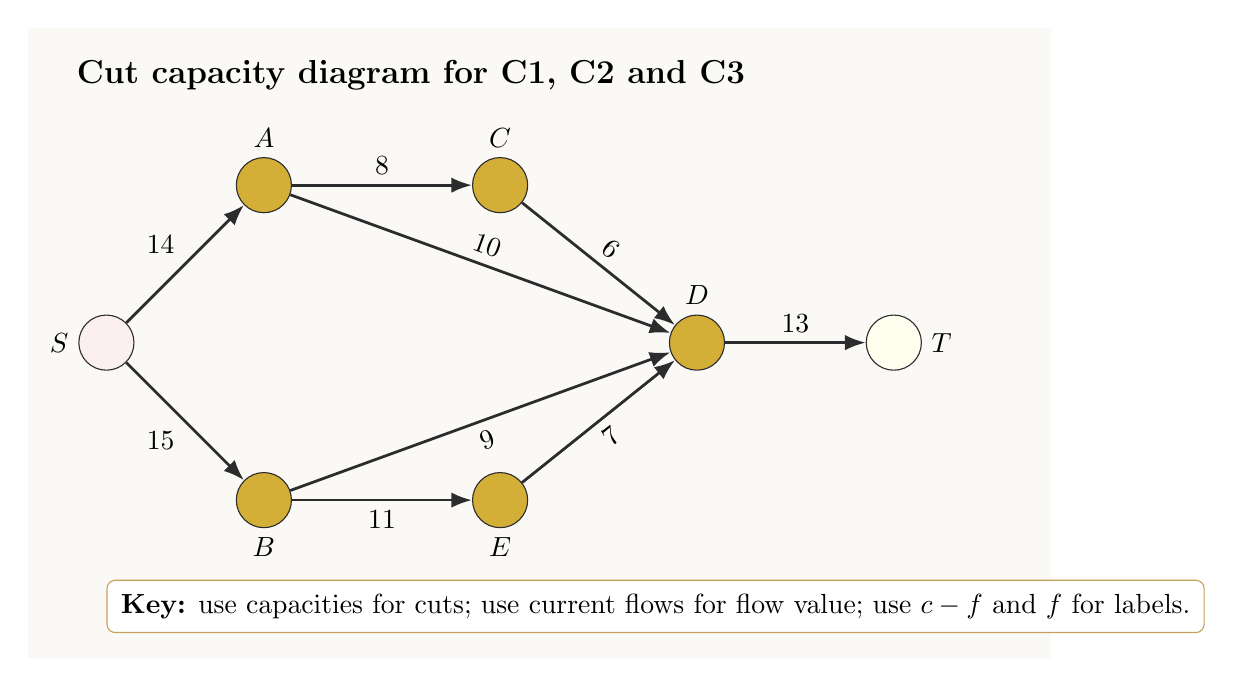
\begin{tikzpicture}[>=Latex, vertex/.style={circle,draw=Line,fill=Gold,minimum size=7mm}, arc/.style={->,draw=Line,line width=1pt}, note/.style={draw=MutedGold,fill=white,rounded corners=3pt,align=left,inner sep=5pt}]
\fill[Canvas] (-1,-1) rectangle (12,7);
\node[font=\large\bfseries,anchor=west] at (-.5,6.4) {Cut capacity diagram for C1, C2 and C3};
\node[vertex,fill=SoftRose,label=left:$S$] (S) at (0,3) {};
\node[vertex,label=above:$A$] (A) at (2,5) {};
\node[vertex,label=below:$B$] (B) at (2,1) {};
\node[vertex,label=above:$C$] (C) at (5,5) {};
\node[vertex,label=below:$E$] (E) at (5,1) {};
\node[vertex,label=above:$D$] (D) at (7.5,3) {};
\node[vertex,fill=Ivory,label=right:$T$] (T) at (10,3) {};
\draw[arc] (S)--node[above left]{14} (A);
\draw[arc] (S)--node[below left]{15} (B);
\draw[arc] (A)--node[above]{8} (C);
\draw[arc] (A)--node[sloped,above]{10} (D);
\draw[arc] (B)--node[sloped,below]{9} (D);
\draw[arc] (B)--node[below]{11} (E);
\draw[arc] (C)--node[sloped,above]{6} (D);
\draw[arc] (E)--node[sloped,below]{7} (D);
\draw[arc] (D)--node[above]{13} (T);
\node[note,anchor=west] at (0,-.35) {\textbf{Key:} use capacities for cuts; use current flows for flow value; use $c-f$ and $f$ for labels.};
\end{tikzpicture}
\end{document}
